\chapter{Analisis Penyelesaian Masalah}
\label{chLanalisis}

Pada bab analisis masalah ini akan dibahas mengenai masalah yang akan diselesaikan beserta solusi yang ditawarkan. Selain itu bab ini juga akan membahas tentang contoh penyelesaian masalah dengan data yang skalanya lebih kecil. 

\section{Analisis Masalah}
\label{sec: Analisis Masalah}

Perkembangan dunia \web selama lima tahun terakhir sangat pesat. Pesatnya perkembangan dunia \web ini didukung oleh munculnya berbagai macam teknologi yang dapat digunakan untuk membuatnya. Banyaknya teknologi yang bermunculan ini tentunya digunakan untuk membuat \web semakin baik dari sisi performa maupun pengalaman pengguna \web. Perkembangan dari penggunaan teknologi ini kemudian dicatat oleh sebuah situs bernama \http. Situs ini menyediakan data yang mencatat berbagai matriks penilaian yang dapat mengukur baik maupun buruknya performa sebuah \web. Data yang disajikan tentunya tidak mudah untuk dimengerti oleh semua orang. 

Solusi yang ditawarkan untuk mempermudah pengguna data untuk mengerti data yang disajikan adalah dengan cara melakukan visualisasi yang sesuai. Visualisasi yang dilakukan juga dapat disesuaikan dengan kebutuhan dari pengguna sehingga visualisasi yang digunakan akan berupa visualisasi yang interaktif. Data yang sudah didapatkan kemudian diolah dengan menggunakan bahasa SQL untuk kemudian hasil \textit{query}. yang menghasilkan potongan data yang dibutuhkan, divisualisasikan ke dalam bentuk visualisasi yang dibutuhkan.

\section{Data Kecil}
\label{sec: datakecil}

Bagian ini akan berisi tentang penyiapan data kecil kemudian setelah itu akan dilanjutkan dengan melakukan pengolahan dan visualisasi dengan menggunakan data kecil.

\subsection{Penyiapan Data Kecil}
\label{subsec:penyiapan data kecil}

Data kecil yang digunakan merupakan data \textit{sample} yang diberikan oleh \http. Data yang digunakan berasal dari data yang sudah diperbaharui oleh \http. Data yang didapatkan adalah data dari tanggal 1 Februari 2024 sampai dengan 1 Februari 2025. Data yang digunakan akan lebih berfokus pada tanggal, teknologi, \textit{client}, dan url utama dari halaman \web, sehingga kolom dan baris lainnya tidak akan digunakan. Pengumpulan data dilakukan dengan melakukan \textit{query} dengan menggunakan \textit{Google Big Query}. Hasil dari \textit{query} tadi kemudian disimpan ke dalam format CSV (\textit{Comma Separated Value}). Salah satu query yang dapat digunakan untuk mengumpulkan data dapat dilihat pada Kode~\ref{kode:kumpuldatakecil}. Kode tersebut akan mengembalikan data yang berisi kolom \textit{date, client, root\_page}, dan \textit{technology} yang berasal dari tabel \textit{pages} dan data yang diambil berasal dari rentang waktu yang sudah disebutkan sebelumnya namun, data dibatasi 10.000.000 baris.

\begin{lstlisting}[language=SQL, caption=Kode untuk mengumpulkan data kecil, label=kode:kumpuldatakecil]

    SELECT DISTINCT date, client, root_page, t.technology,  
    FROM `httparchive.crawl.pages`, UNNEST(technologies) as t 
    WHERE date BETWEEN "2024-02-01" and "2025-02-01" limit 100000000
    
\end{lstlisting}

\subsection{Pengolahan Data Kecil}
\label{subsec:pengolahankecil}
Setelah data yang akan digunakan siap, hal selanjutnya adalah mengolah data tersebut. Pengolahan data ini akan menggunakan bahasa \textit{Python}. DAlam pengolahan ini perspektif yang dilihat 

\subsubsection{Perkembangan Sepuluh Teknologi Populer}
Hal pertama yang dilakukan adalah dengan memuat data \textit{sample}. Contoh dari data \textit{ sample} yang dimuat dapat dilihat pada Tabel~\ref{tab:sample}. Data tersebut berisikan tanggal diambilnya data, perangkat yang digunakan untuk mengambil data, url utama dari halaman \web yang dites, dan teknologi yang digunakan oleh halaman \web yang dites.
\begin{table}[H]
    \centering
    \caption{Lima baris data \textit{sample}}
    \label{tab:sample}
    \begin{tabular}{|l|l|l|l|}
        \hline
        date & client & root\_page & technology \\ \hline
        2025-02-01 & desktop & https://www.schilling-rechtsanwalt.com/ & Google Analytics \\ \hline
        2025-02-01 & mobile & https://kiztopia.co.id/ & HSTS \\ \hline
        2025-02-01 & mobile & https://ca.brixton.com/ & Klaviyo \\ \hline
        2025-02-01 & mobile & https://spinfinity.casino/ & Gatsby \\ \hline
        2025-02-01 & mobile & http://namhaerun.com/ & YouTube \\ \hline
    \end{tabular}
\end{table}

Setelah itu kemudian data dikelompokkan berdasarkan teknologinya dengan menggunakan \textit{method} \verb|Group By|. Contoh hasil dari pengelompokan data ini dapat dilihat pada Tabel~\ref{tab:gbsample}. Terlihat bahwa untuk tanggal yang sama ada berbagai teknologi dengan jumlah pemakaian dari berbagai halaman \web yang beragam. Data yang dikelompokan juga berasal dari penggunaan teknologi untuk perangkat \mobile dan \desktop.
\begin{table}[H]
    \centering
    \caption{Contoh hasil pengelompokan data \textit{sample} berdasarkan teknologi yang digunakan}
    \label{tab:gbsample}
    \begin{tabular}{|l|l|l|}
        \hline
        date & technology & jumlah pemakaian \\ \hline
        2024-02-01 & Datadog & 4591 \\ \hline
        2024-02-01 & Node.js & 14794 \\ \hline
        2024-02-01 & Google Tag Manager & 124814 \\ \hline
        2024-02-01 & Sendgrid & 12152 \\ \hline
        2024-02-01 & Dojo & 2087 \\ \hline
    \end{tabular}
\end{table}

Kemudian data yang sudah terkelompok diurutkan berdasarkan penggunaan paling banyak. Contoh hasil pengurutan ini dapat dilihat pada Tabel~\ref{tab:urutgbsample}. Terlihat bahwa teknologi yang paling banyak digunakan pada rentang waktu 1 Februari 2024 sampai 1 Februari 2025 adalah \textit{JQuery} dengan 4464436 halaman \web yang menggunakan teknologi ini untuk membangunnya.
\begin{table}[H]
    \centering
    \caption{Contoh data penggunaan teknologi yang sudah diurutkan berdasarkan pemakaian paling banyak}
    \label{tab:urutgbsample}
    \begin{tabular}{|l|l|}
        \hline
        technology & Jumlah Pemakaian \\ \hline
        jQuery & 4464436 \\ \hline
        Open Graph & 3834676 \\ \hline
        Google Analytics & 3323217 \\ \hline
        PHP & 3294059 \\ \hline
        Google Font API & 2802138 \\ \hline
        core-js & 2573059 \\ \hline
    \end{tabular}
\end{table}

Setelah itu sepuluh teknologi yang paling banyak digunakan akan diambil. Setelah sepuluh teknologi yang populer sudah didapatkan, Hal selanjutnya yang dicari adalah penggunaan sepuluh teknologi tersebut dalam rentang waktu yang sudah ditentukan. Setelah itu hal yang dilakukan adalah memvisualisasikan data yang sudah didapatkan. Hasil visualisasinya dapat dilihat pada Gambar~\ref{fig:sample10}. Terlihat dari hasil visualisasinya bahwa untuk semua teknologi mengalami penurunan pemakaian pada tanggal 1 mei 2024. Selain itu semua teknologi terlihat memiliki perkembangan yang hampir mirip dan stabil.
\begin{figure}[H]
    \centering
    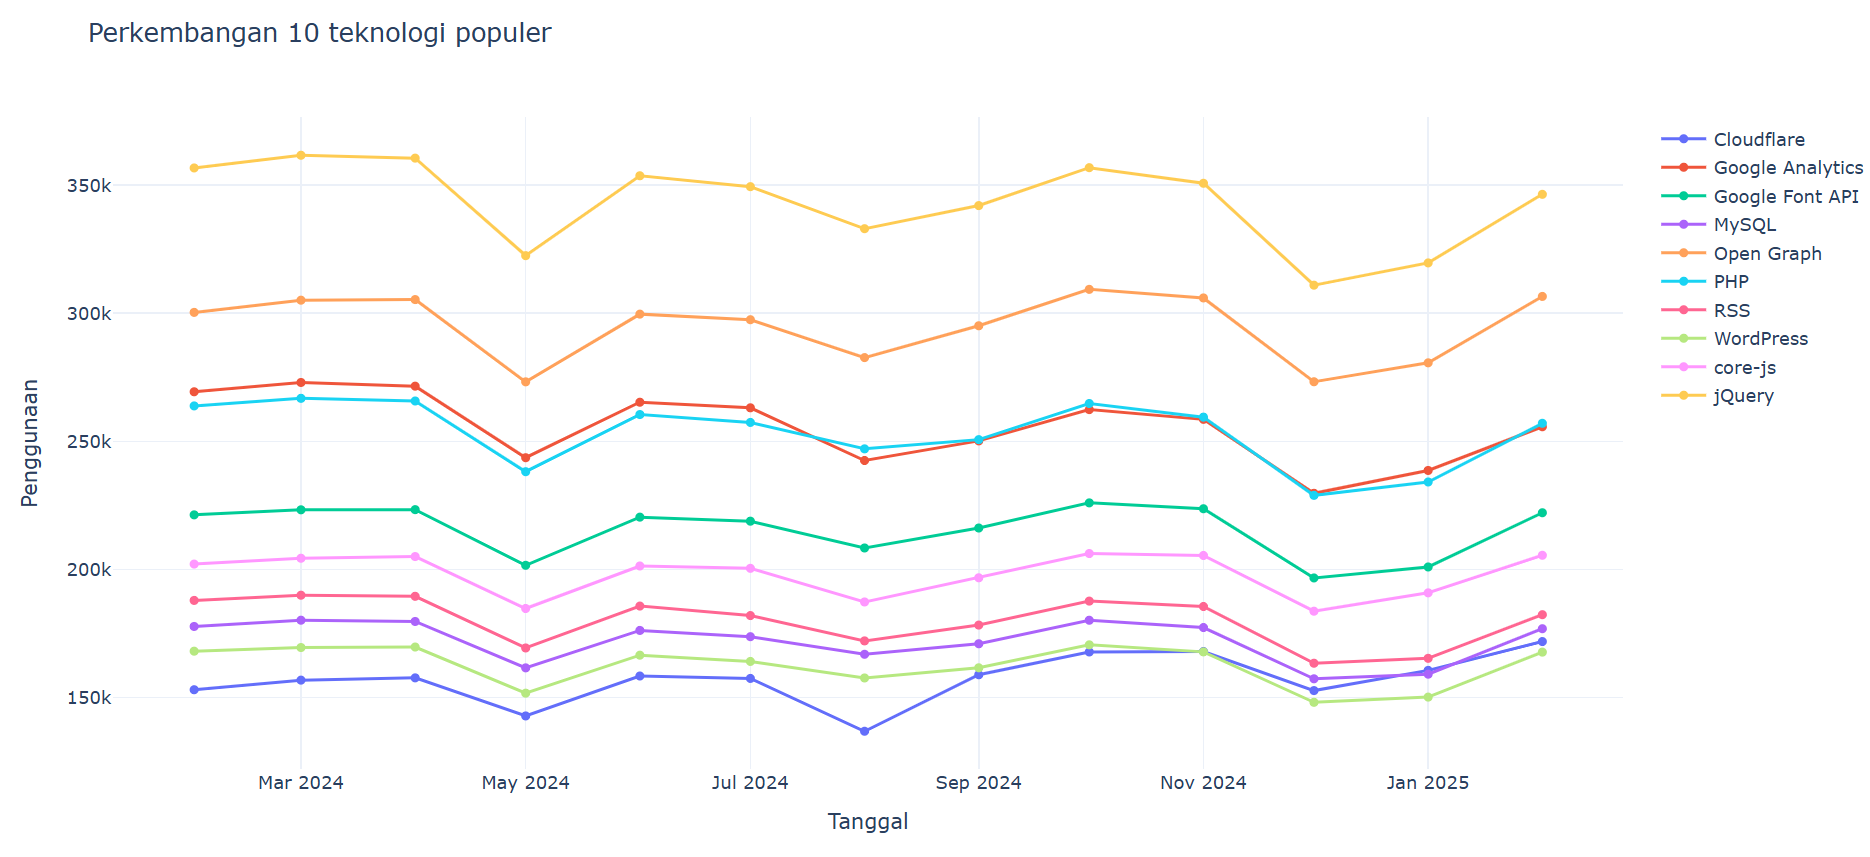
\includegraphics[width=0.7\linewidth]{Gambar/Perkembangn 10 teknologi populer.png}
    \caption{Perkembangan sepuluh teknologi populer berdasarkan jumlah halaman \web}
    \label{fig:sample10}
\end{figure}
